\tikzset{
	A/.pic={
        code={
\draw[black](0,0)node[rotate=00]{\small \texttt{CMakeFiles $\dagger$}};
\draw[black](0,-0.5)node[rotate=00]{\tiny \texttt{...}};
\draw[black](0,-0.9)node[rotate=00]{\tiny \texttt{...}};
\draw[black](0,-1.3)node[rotate=00]{\tiny \texttt{...}};
%\draw[black,thick](-0.5,-0.15)rectangle(0.5,0.15);   
							}
	}
}

\tikzset{
	C/.pic={
        code={
\draw[black](0,0)node[rotate=00]{\small \texttt{Bin-dir $\dagger$}};
\draw[black](0,-0.5)node[rotate=00]{\tiny \texttt{binaries}};
\draw[black](0,-0.9)node[rotate=00]{\tiny \texttt{executable}};
\draw[black](0,-1.3)node[rotate=00]{\tiny \texttt{...}};
%\draw[black,thick](-0.5,-0.15)rectangle(0.5,0.15);   
							}
	}
}


\tikzset{
	B/.pic={
        code={
\draw[black](0,0)node[rotate=00]{\small \texttt{Src-dir}};
\draw[black](0,-0.5)node[rotate=00]{\tiny \texttt{.cpp-files}};
\draw[black](0,-0.9)node[rotate=00]{\tiny \texttt{additional}};
\draw[black](0,-1.3)node[rotate=00]{\tiny \texttt{CMakeLists.txt}};
						}
	}
}

\tikzset{
	F/.pic={
		code={
			\draw[black](0,0)node[rotate=00]{\small \texttt{Test-dir}};
			\draw[black](0,-0.5)node[rotate=00]{\tiny \texttt{my Test}};
			\draw[black](0,-0.9)node[rotate=00]{\tiny \texttt{.cpp-filesl}};
			\draw[black](0,-1.3)node[rotate=00]{\tiny \texttt{...}};
		}
	}
}



\tikzset{
	E/.pic={
        code={
\draw[black](0,0)node[rotate=00]{\small \texttt{Header-dir}};
\draw[black](0,-0.5)node[rotate=00]{\tiny \texttt{.hpp-files:}};
\draw[black](0,-0.9)node[rotate=00]{\tiny \texttt{...}};
\draw[black](0,-1.3)node[rotate=00]{\tiny \texttt{...}};
							}
	}
}




\tikzset{
	D/.pic={
		code={
			\draw[black](0,0)node[rotate=00]{\small \texttt{Lib-dir $\dagger$}};
			\draw[black](0,-0.5)node[rotate=00]{\tiny \texttt{...}};
			\draw[black](0,-0.9)node[rotate=00]{\tiny \texttt{...}};
			\draw[black](0,-1.3)node[rotate=00]{\tiny \texttt{...}};
			}
	}
}

\tikzset{
	G/.pic={
		code={
			\draw[black](0,0)node[rotate=00]{\small \texttt{Testing-dir $\dagger$}};
			\draw[black](0,-0.5)node[rotate=00]{\tiny \texttt{...}};
			\draw[black](0,-0.9)node[rotate=00]{\tiny \texttt{...}};
			\draw[black](0,-1.3)node[rotate=00]{\tiny \texttt{...}};
		}
	}
}



\tikzset{
	main/.pic={
        code={
%\draw[black](0,0.25)node[rotate=00]{\tiny \texttt{Project-dir}};
\draw[black](0,0)node[rotate=00]{\small \texttt{Example-dir}};
\draw[black](0,-0.5)node[rotate=00]{\small \texttt{CMakeLists.txt}};
\draw[black](0,-0.9)node[rotate=00]{\small \texttt{Make}};
%\draw[black](0,-1.3)node[rotate=00]{\small \texttt{...}};
%\draw[black](0,0)node[rotate=00]{\small \texttt{MakeLists.txt}};
%\draw[black,thick](-0.5,-0.15)rectangle(0.5,0.15);   
						}
	}
}

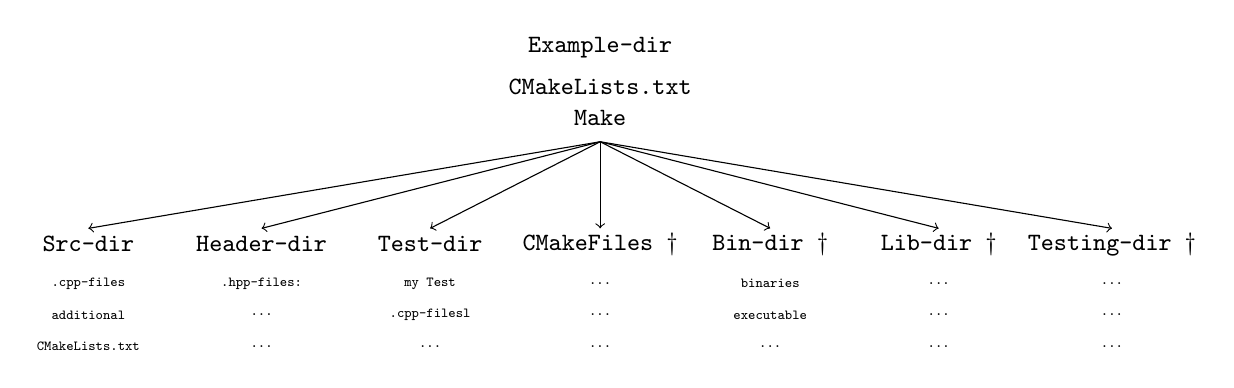
\begin{tikzpicture}
%Gitter
%\draw[step=0.5cm,very thin,black!20] (-6,-6) grid(6,6);
%\draw(-6,0)--(6,0);
%\draw(0,6)--(0,-6);

\path (0,4.5) pic {main};
\path (-6.5,2) pic {B};
\path (-4.3,2) pic {E};
\path (-2.16,2) pic {F};
\path (0,2) pic {A};
\path (2.16,2) pic {C};
\path (4.3,2) pic {D};
\path (6.5,2) pic {G};

\draw [black,->] (0,3.3)--(-6.5,2.2);
\draw [black,->] (0,3.3)--(-4.3,2.2);
\draw [black,->] (0,3.3)--(-2.16,2.2);
\draw [black,->] (0,3.3)--(0,2.2);
\draw [black,->] (0,3.3)--(2.16,2.2);
\draw [black,->] (0,3.3)--(4.3,2.2);
\draw [black,->] (0,3.3)--(6.5,2.2);
\end{tikzpicture}

